\documentclass[a4paper,11pt]{article}
\usepackage{amsmath,amssymb,amsfonts,latexsym}
\usepackage[utf8]{inputenc}
\usepackage{fancyvrb}
\usepackage{graphicx}
\usepackage[margin=1.1in]{geometry}
\usepackage{url}
\usepackage{verbatim}
\usepackage{fixltx2e}
\usepackage{amsfonts}
\usepackage{amssymb}
\usepackage{amsmath}
\usepackage{float}
\usepackage{listings}
\usepackage{lmodern}
\usepackage[spanish]{babel}
\lstset{frame=tb,
  language=Java,
  aboveskip=3mm,
  belowskip=3mm,
  showstringspaces=false,
  columns=flexible,
  basicstyle={\small\ttfamily},
  numbers=none,
  breaklines=true,
  breakatwhitespace=true
  tabsize=3
}
\title{Speech compression \\
M\'etodos Num\'ericos Avanzados}
\author{Enzo Altamiranda, Cristian Ontiver, Valeria Serber}
\date{\today}
\begin{document}

\maketitle
\thispagestyle{empty}
\vspace{3cm}

\renewcommand{\abstractname}{Resumen}
\begin{abstract}
El siguiente informe explora el uso de la transformada rápida de Fourier, en
combinación con la codificación de Huffman para la compresión de voz. Se
realiza un estudio comparativo de diferentes niveles de cuantificación y sus
efectos tanto en el tamaño como la calidad - en términos de distorción - del
archivo comprimido.
\end{abstract}
\section{Palabras Clave}
Transformada Rápida de Fourier, Compresión de voz, Codificación de Huffman
\newpage
\section{Introducci\'on}
\begin{comment}
[Introduce el tema contextualizando la informacion. Puede incluirse un parrafo
con una breve descripcion historica, otro parrafo motivando el tema. El ultimo
parrafo de esta seccion tiene que ser la descripcion de la estructura del
artıculo, explicitando en que seccion se trata cada tema.]
\end{comment}
La voz, entendida como el sonido generado por el aparato fonador humano, se
encuentra en frencuencias de entre $80$ a $1100$ Hz.  Teniendo esto en cuenta,
a la hora de almacenar digitalmente una señal de voz, es posible utilizar
métodos para reducir el tamaño necesario para guardar la información
correspondiente a esta señal.\\
Tradicionalmente estos se dividen en dos. Por un lado métodos "lossless" (sin
pérdida), es decir, métodos que almacenan la información de modo tal que esta
pueda ser recuperada en su totalidad. Por otro, métodos "lossy" (con pérdida),
en los cuales, tomando ventaja de que el rango de audición humano suele
situarse entre los $20$ y $20.000$ Hz (con variaciones de individuo a
individuo), descartan información considerada redundante (aquella por encima o
por debajo de ese rango).\\
Aquí exploramos una forma de lograr lo segundo, mediante el uso de la
transformada rápida de Fourier, en conjunto con la codificación de Huffman,
para lograr almacenar diferentes archivos de sonidos conteniendo voces, de
manera que se reduzca el tamaño necesario.\\
Como se verá más adelante, una reducción en la distorición y aumento en la
fidelidad del audio comprimido implican la necesidad de mayor información, y
por ende, una menor reducción en relación al tamaño (en bytes) original.
\newpage
\section{Metodolog\'ia}
\begin{comment}
[Hay que relatar los pasos que se fueron realizando, incluyendo los modelos
utilizados, los analisis hechos, las pruebas realizadas.]
\end{comment}
\subsubsection{Grabación de voz\'on}
Mediante el programa Audacity\textsuperscript{TM}, se grabaron treinta muestras
de diferentes personas, pronunciando desde palabras individuales, a frases más
elaboradas. Las mismas se almacenaron en el formato sin compresión WAV, con un
solo canal de audio (mono), y una frecuencia de muestreo de $8$ Khz.
\subsubsection{Obtención de la señal de los wav}
Para obtener la señal de los archivos se utilizó la función \verbatim+wavread+ de octave,
la cual dado un archivo de audio mono, retorna un vector con las muestras.
\subsubsection{Transformada de Fourier y truncado}
En base a la función \verbatim+fft+ de octave, se calculó la Transformada Rápida de
Fourier de cada archivo, obteniendo la señal en frecuencia a comprimir.
Debido a que la señal de audio de un wav es real, se pudo truncar el vector
obtenido de la \verbatim+fft+, conservando solo la mitad más uno de los valores. Esto se
debe a que, sea $X[n]$ una función discreta tal que $X[n] \in
\mathbb{R}$, y sea $N$ el número de muestras totales, entonces:
\begin{equation} \label{eq1}
    \begin{split}
        \hat{X}[k] & = \hat{X}[((-k))_N] \\
         & = \hat{X}[((N - k))_N] \\
         & = \hat{X}[N-k] \\
     \end{split}
\end{equation}
Donde se usa la notación $((a))_b$ para denotar $a$ módulo $b$.
Luego:
\begin{equation} \label{eq2}
    \begin{split}
        \hat{X}[k] & = \hat{X}[N-k] \\
        \hat{X}[\frac{N}{2}] & = \hat{X}[N-\frac{N}{2}] \\
        \hat{X}[\frac{N}{2}+1] & = \hat{X}[N-\frac{N}{2}+1] \\
     \end{split}
\end{equation}
\subsubsection{Eliminación de coeficientes próximos a cero}
Para cierto valor $\epsilon$ que se fue variando arbitrariamente, se reemplazó
los valores de $\hat{X}[k]$ tales que $|\hat{X}[k]| < \epsilon$, por cero. \\
Esto permitió reducir el tamaño final mejorando el proceso de compresión,
eliminando señales débiles que poco aportan al sonido en su totalidad.
\subsection{Cuantificación y ``thresholding''}
Cuantificar una señal implica asociar (``mappear'') el conjunto de valores de la
misma a uno menor. Esto, como es de esperarse, tiene la finalidad de
reducir el tamaño final del archivo comprimido. Existen varios métodos de
cuantificación, desde simples a otros más complejos que toman en cuenta la
capacidad humana para distinguir frecuencias muy similares, de forma de agrupar
estas bajo una misma y así reducir la información necesaria a almacenar sin una
pérdida de fidelidad significativa. En nuestro caso, hicimos uso de una
cuantificación lineal, donde el paso $\Delta$ de la misma se obtienen
mediante la fórmula:
$$\Delta = \left(\frac{M_{max} - M_{min}}{L}\right)$$
Siendo $M_{max}$ el máximo valor en el vector de señales, $M_{min}$ el mínimo,
y $L$ el nivel de cuantificación deseado.
Estos tres valores deben ser almacenados en el archivo comprimido, ya que
aportan información necesaria para la descompresión (en otras palabras, se
requieren para revertir la codificación de Huffman, mencionada en la próxima
sección).
\subsection{Codificación de Huffman}
Finalmente se hace empleo de la codificación de Huffman, la cual asigna
secuencia de bits a cada valor, en base a la frecuencia con que aparece cada
uno. Es decir, aquellos valores con mayor frecuencia son asignados las
secuencias más cortas, codificando de manera eficiente la información y
reduciendo su tamaño.
Para nuestro caso particular, evitamos guardar los archivos codificados en sí,
pero calculamos la misma para saber cuanto ocuparía la versión final
comprimida.
\subsection{Reconstrucción de la señal}
Para reconstruir la señal original desde el archivo cuantificado, se aplican los
procesos inversos. En base a la propiedad mencionada anteriormente por la cual
se pudo descartar la mitad menos uno de los valores, se vuelve a generar los
faltantes, y al vector obtenido se le aplica la función inversa (\verbatim+ifft+
en octave), que, utilizando la antitransformada de Fourier, se genera un archivo
de sonido descomprimido, similar al original (no idéntico, debido al descarte de
valores y aproximaciones). Notar que si efectivamente se realiza la
codificación de Huffman, se requieren los tres parámetros mencionados
previamente durante la cuantificación, para la decodificación.
\section{Resultados}
A continuación se presentan comparaciones de diferentes archivos de audio, con
su tamaño original, tamaño comprimido, razón de compresión, y distorción.
\begin{center}
    \begin{tabular}{| c | c | c | c | c |}
        \hline
        Archivo & Tamaño (bytes) & Tamaño comprimido (bytes) & Compresión (\%) &  Distorción \\ \hline
        p1.wav & 64700 & 7726 & 0.11941 & 9.4042e-04 \\
        p2.wav & 156684 & 21617 & 0.13797 & 8.6123e-05 \\
        p3.wav & 47404 & 6793 & 0.14328 & 2.6806e-04 \\
        p4.wav & 39468 & 5358 & 0.13574 & 2.8885e-05 \\
        p5.wav & 36644 & 4420 & 0.12062 & 1.8816e-04 \\
        p6.wav & 36644 & 4796 & 0.13086 & 6.1311e-04 \\
        p7.wav & 52748 & 5707 & 0.10818 & 7.0363e-04 \\
        p8.wav & 45428 & 6159 & 0.13556 & 3.1064e-04 \\
        p9.wav & 52748 & 5499 & 0.10424 & 7.9479e-04 \\
        p10.wav & 46892 & 4749 & 0.10127 & 1.0548e-03 \\
        \hline
    \end{tabular}
\end{center}

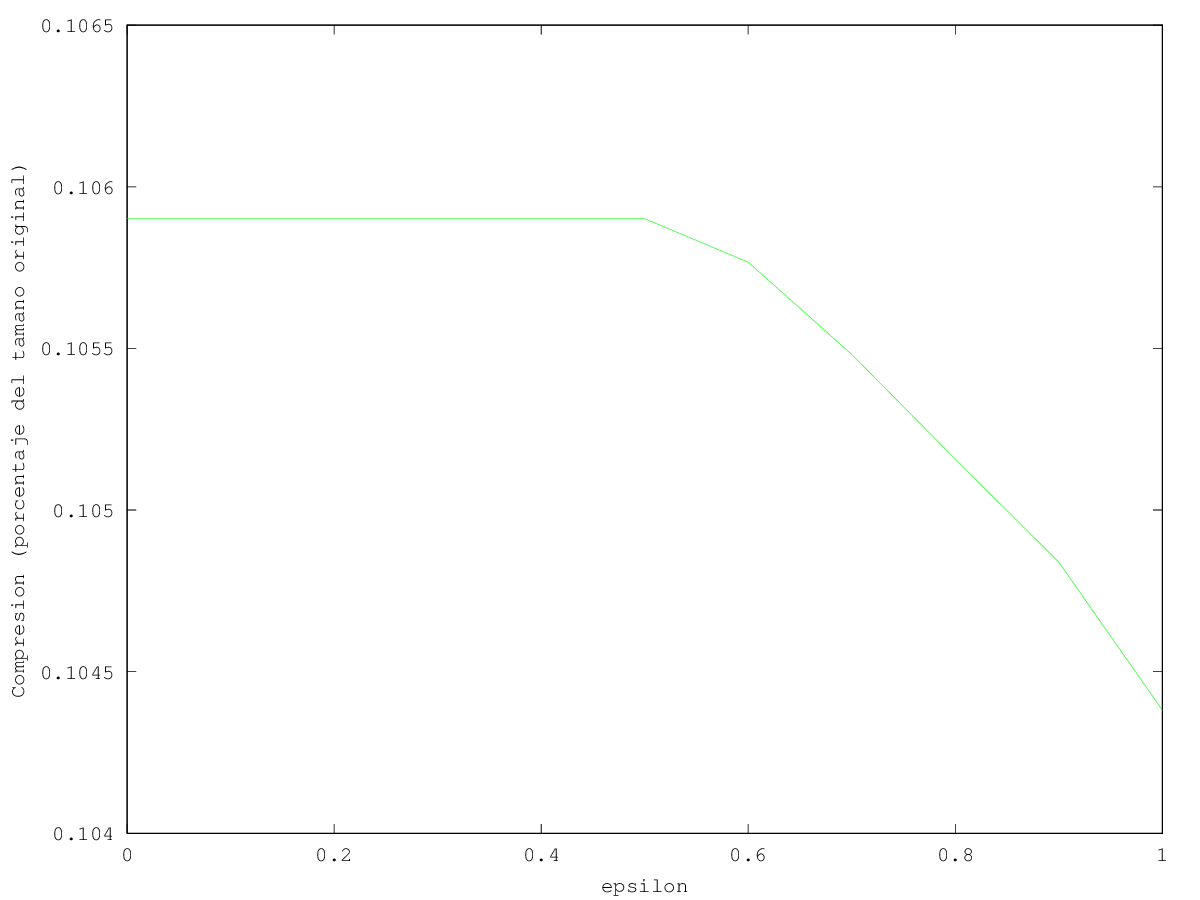
\includegraphics[scale=0.8]{compresion_media_fixed_bits.png}
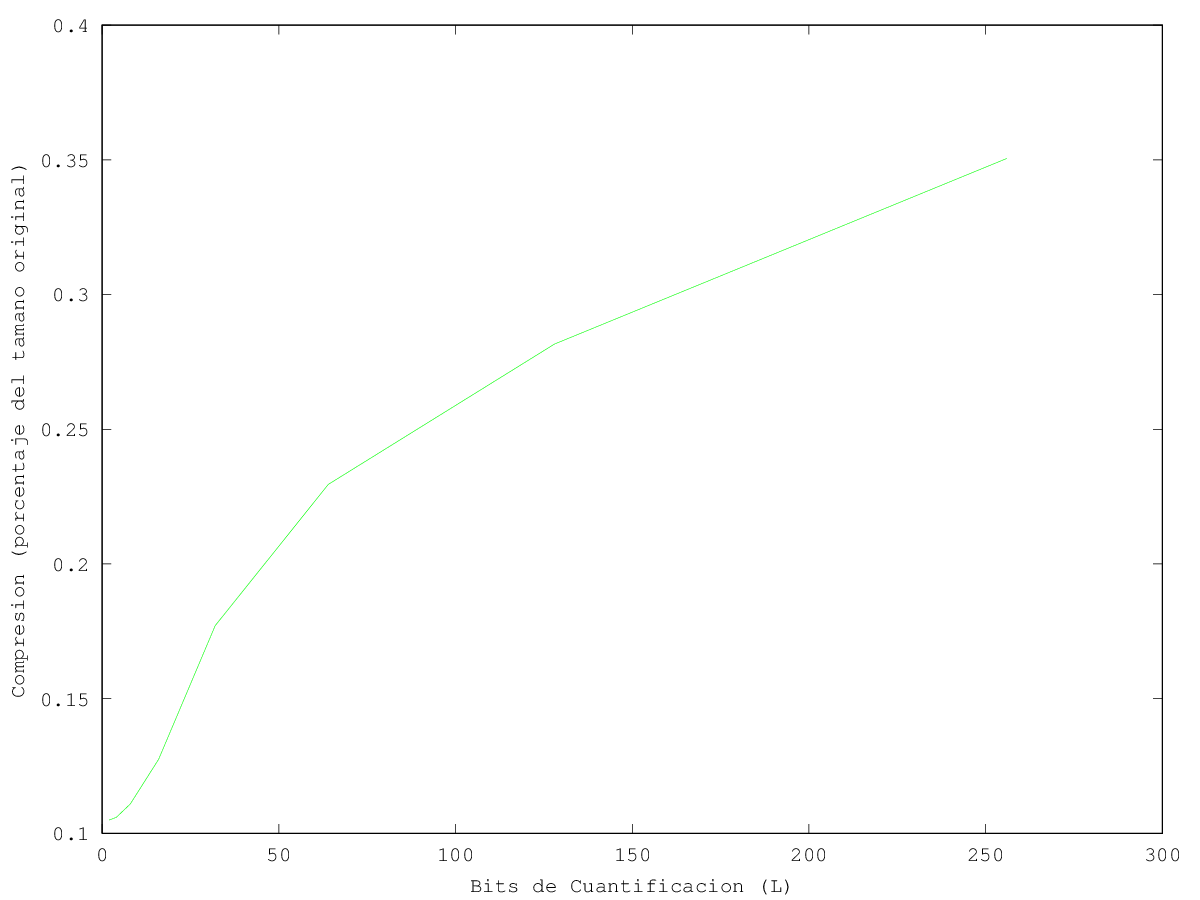
\includegraphics[scale=0.8]{compresion_media_fixed_epsilon.png}
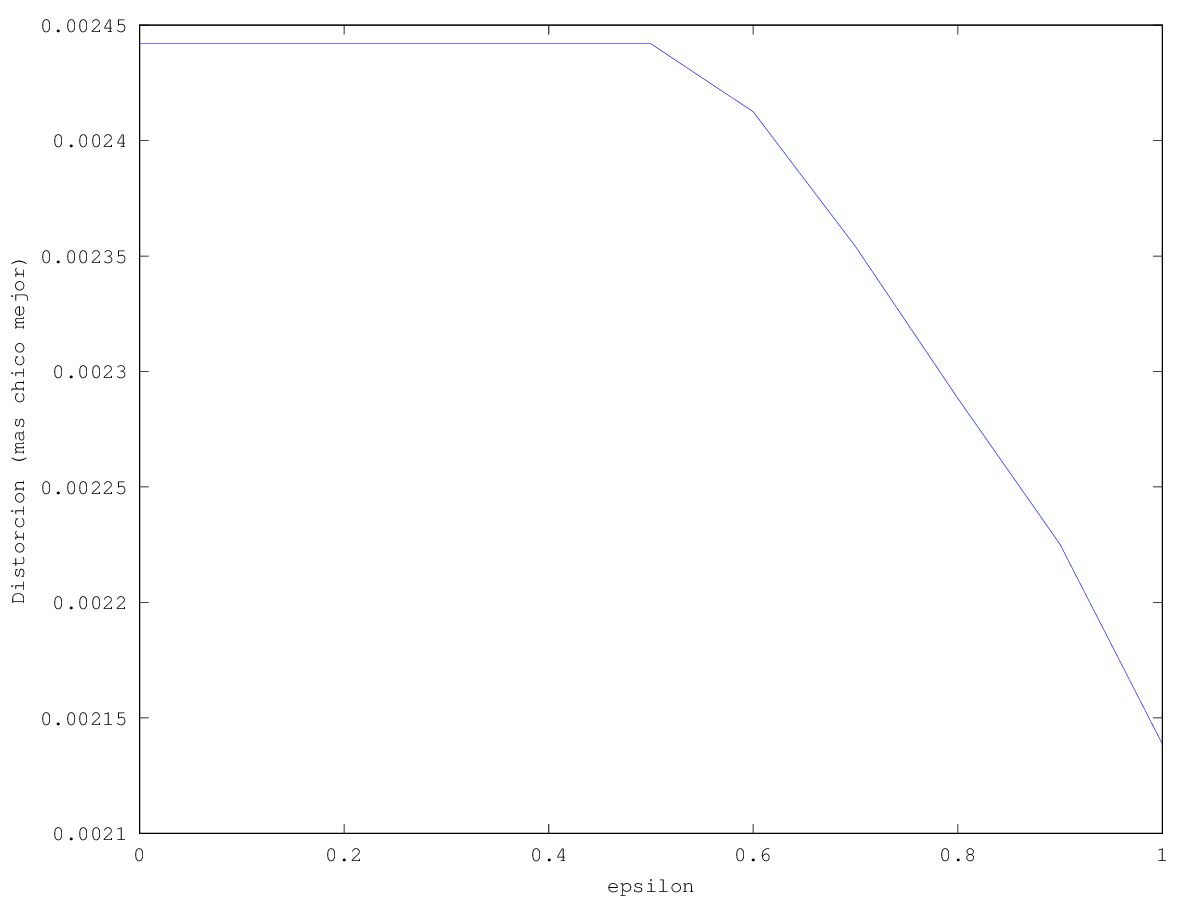
\includegraphics[scale=0.8]{distorcion_media_fixed_bits.png}
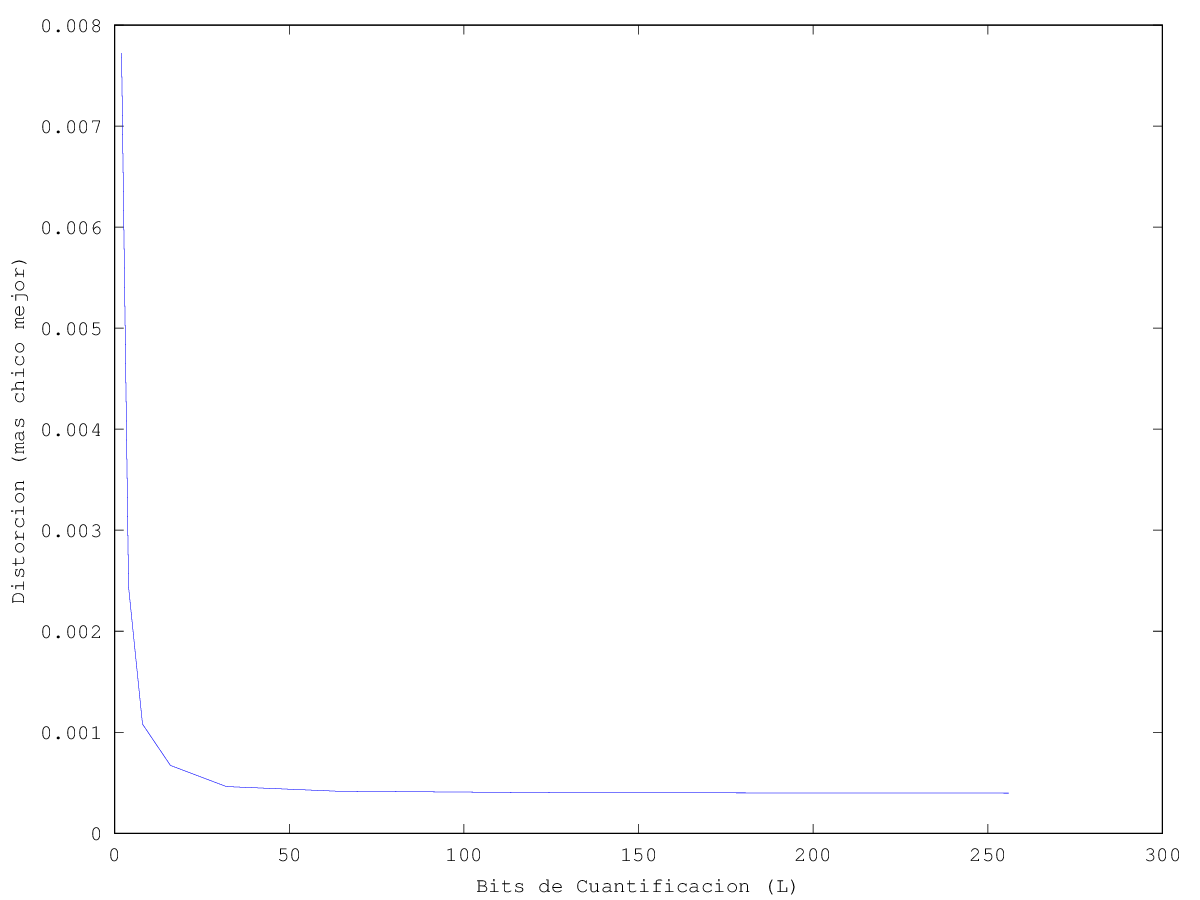
\includegraphics[scale=0.8]{distorcion_media_fixed_epsilon.png}
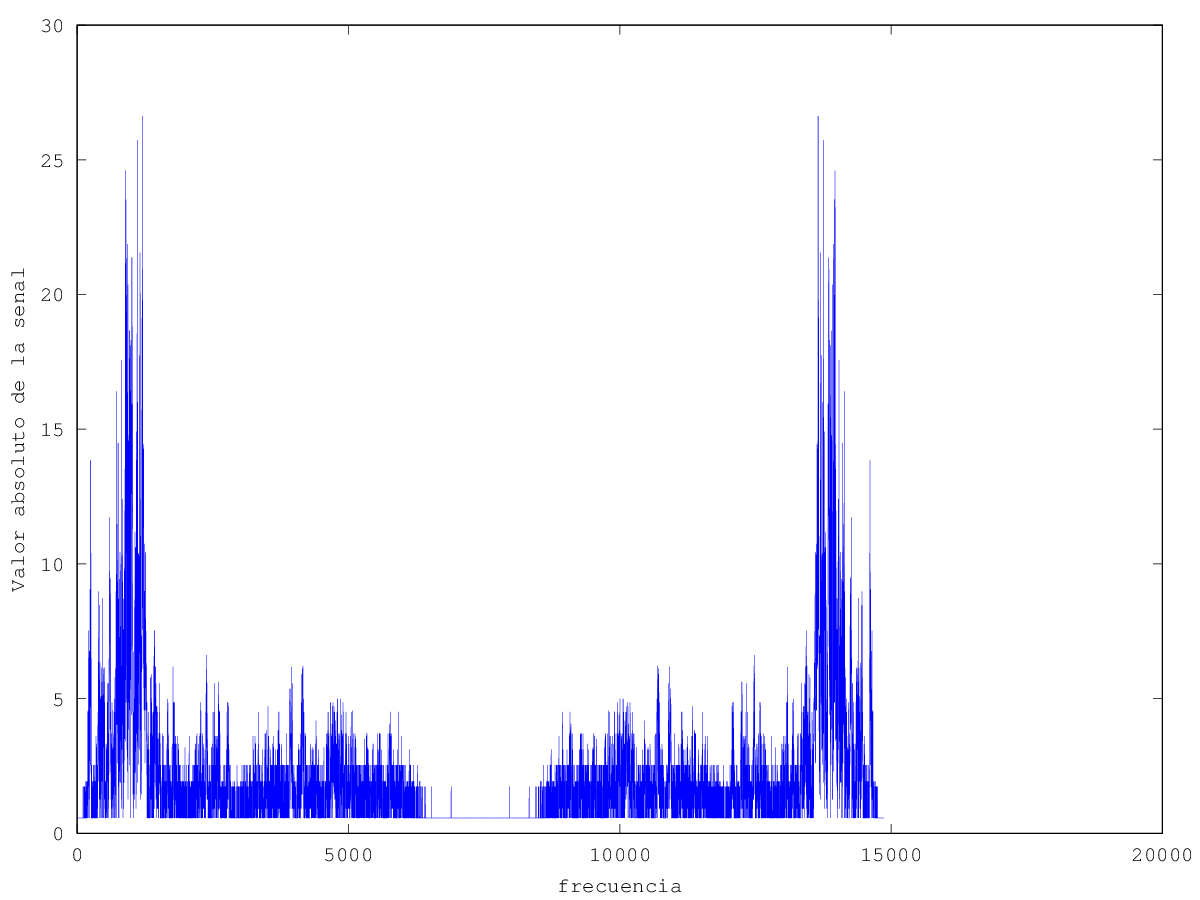
\includegraphics[scale=0.8]{signal_with_compression.png}
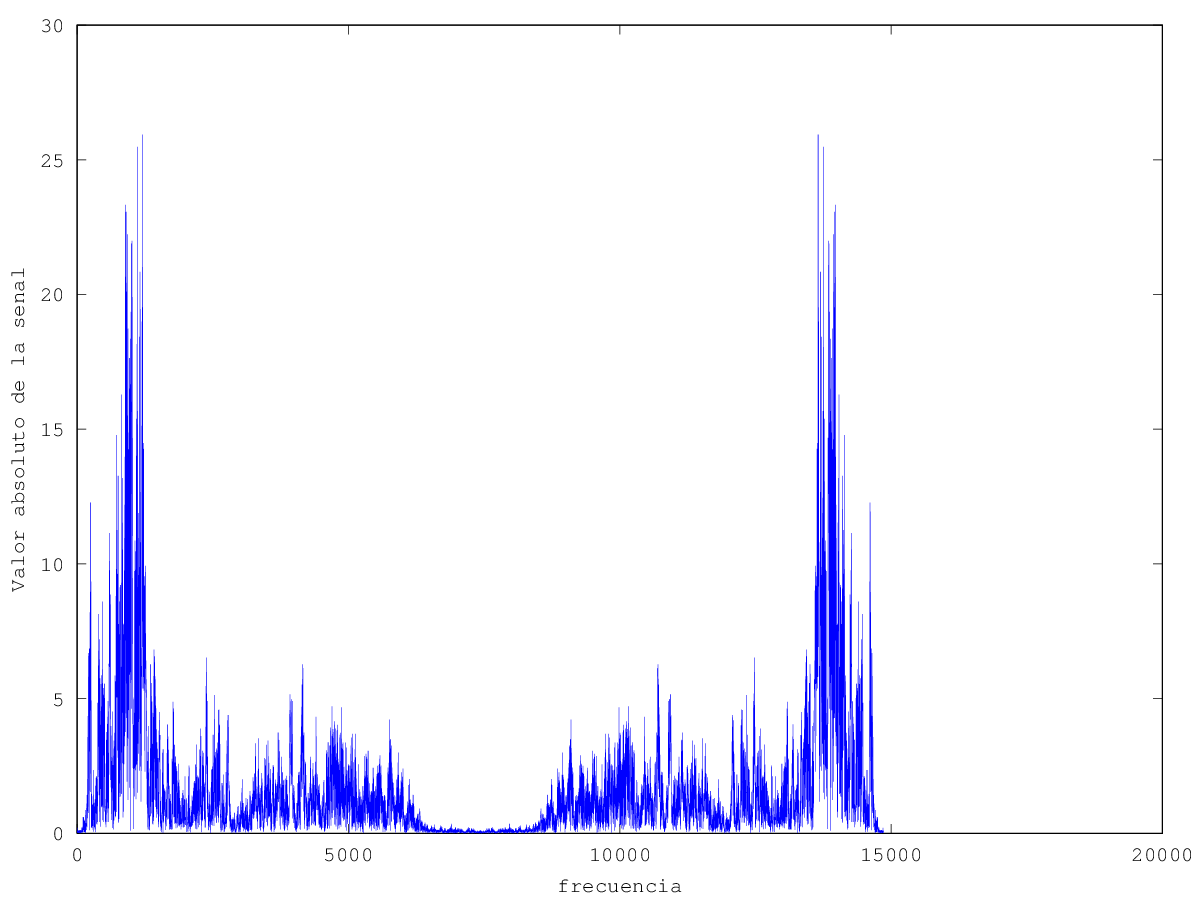
\includegraphics[scale=0.8]{signal_without_compression.png}
\section{Conclusiones}
\newpage
\section{Bibliograf\'ia}
G. Rajesh, A. Kumar, K. Ranjeet. Speech Compression using Different Transform Techniques.
\end{document}
